% !TeX root = ../main.tex

\chapter{Design and Implementation Requirements}\label{chapter:Persistent Threads}

Persistent GPU threads allow the hardware resources to be partitioned and reduce kernel execution and scheduling overhead and are fundamental for other applications seeking to enhance GPU scheduling.  
Many other applications such as coroutines or mega kernels are based on persistent threads as a means of reducing kernel launch overhead and allow further control in application specific scheduling decisions, otherwise black boxed by the cuda api. 
Running persistent threads essentially allows the memory and system configurations to be loaded in ahead of runtime and reduces overhead during execution.

Failing to implement LuisaCompute's coroutines into Apollo, the goal shifted to finding a manual GPU scheduling functionality to implement and use. 
In restricting the scope from GPU coroutines to simply implementing persistent threads into Apollo, this thesis attempted to find an open source implementation which would allow the fine grained scheduling controll specific to Apollo. 
Unfortunately, given that most persistent thread implementations are highly specific they are not open source, which led to selecting an implementation that required more work to make it feasible. 
The only open source persistent thread implementation that was readily available was LightKer, a research project, which measured the hypothetical speedup of using persistent threads over sequential kernel launches. 
Seeking to implement LightKer into Apollo first required a complete restructuring of the code base to support a real time system.

The LightKer implementation itself intended to measure the performance difference between sequential kernel executions versus a persistent kernel implementation.
This implementation constructed simple trivial kernels and tested the overhead difference between calling them explicitely from the host in kernel launches versus implicitely in the persistent kernel. 
Unfortunately, this application does not support variable tasks or memory transfers at runtime, necessary to pass arguments and results back and forth. 
As such, the implementation only succeeds in measuring latency differences between scheduling tasks using a device side while loop versus explicit kernel launches. 
However, the LightKer implementation does provide a simple framework for using a GPU-Host mailbox for scheduling kernel tasks as well as a helpful persistent kernel launch structure. 

\section{Architecture}

From a high level, the architecture implemented into this project appears as follows, with the GPU-Host Mailbox, being used from the Lightkernel project as well as the internal structure.

\begin{figure}[H]
  \centering
  \resizebox{1.0\linewidth}{!}{
	  %\documentclass[tikz, border=5mm]{standalone}
%\usepackage{tikz}
%\usetikzlibrary{shapes, arrows.meta, positioning, decorations.pathreplacing}

%\begin{document}

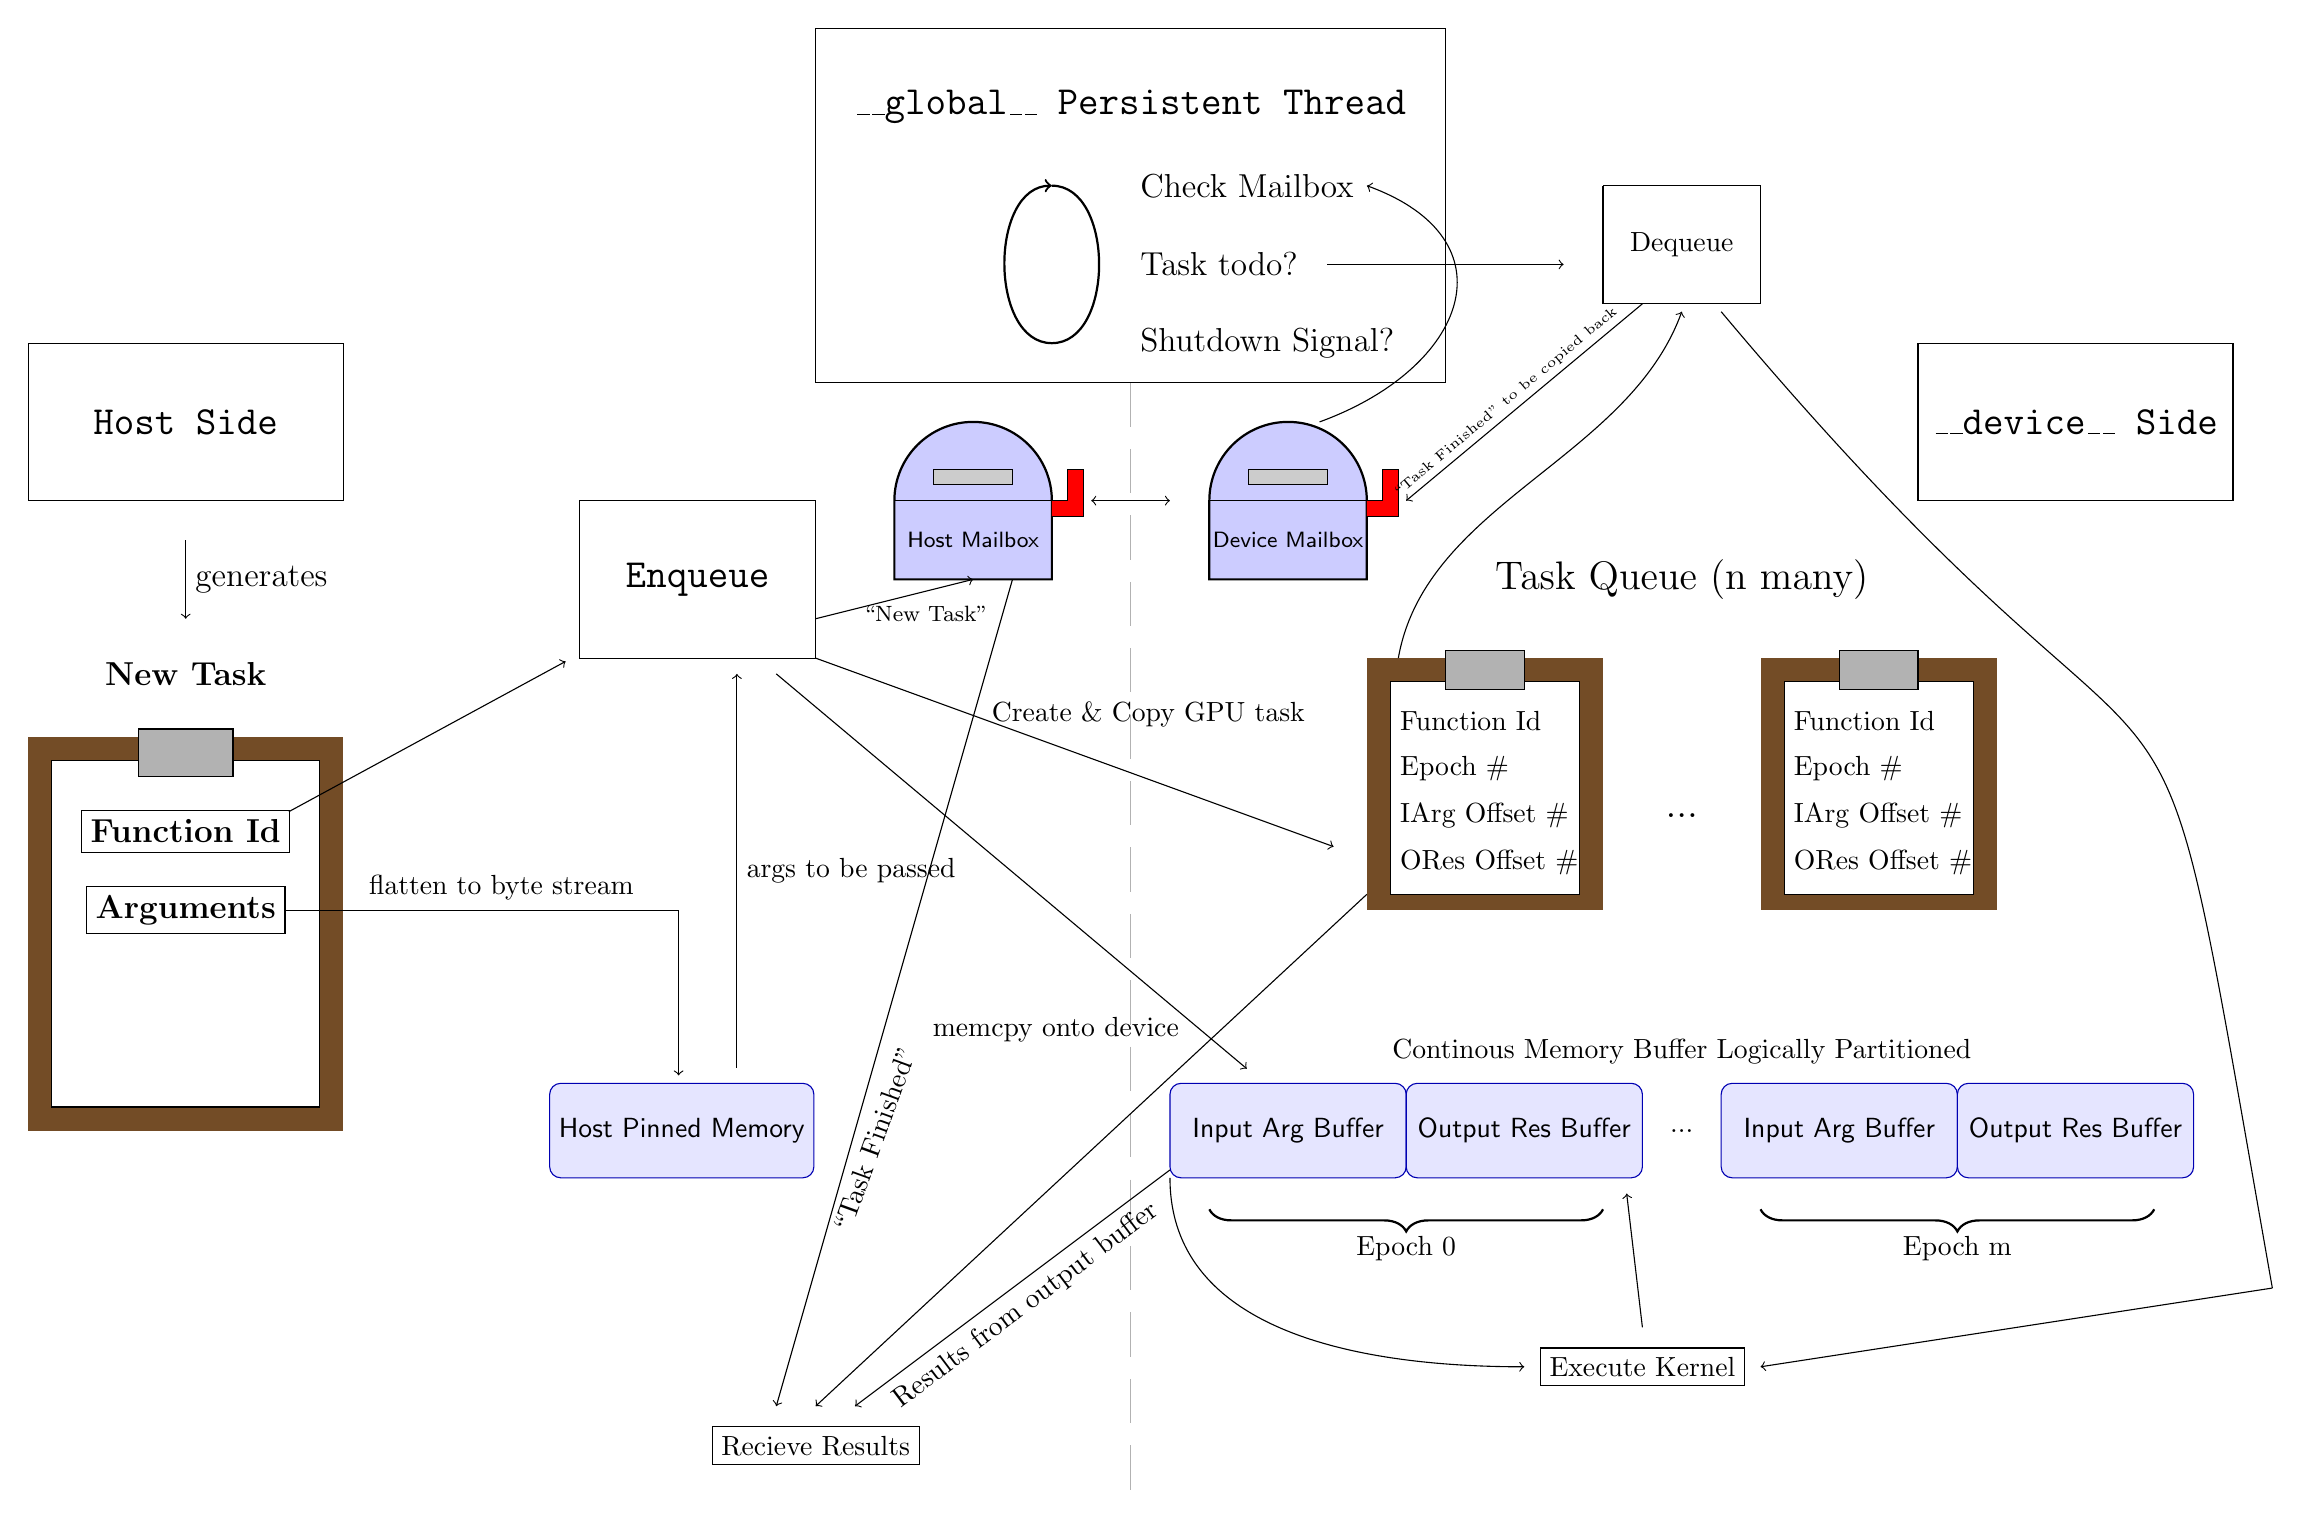
\begin{tikzpicture} [memoryblock/.style={
		draw=blue!70!black, 
		fill=blue!10, 
		rounded corners=4pt, 
		minimum width=3cm, 
		minimum height=1.2cm,
		font=\sffamily
	},
	pinicon/.style={
		symbol/.style={draw, fill=gray!40, symbol color=gray!80, symbol type=pin}
	}
	]

	%\draw[help lines] grid(32,32);


%GLOBAL BOX
	\draw[black] (12,32) -- ++(0:8) -- ++(-90:4.5) -- ++(-180:8) -- ++(-270:4.5);
	\node[minimum size=5] at (16,31) {\Large \texttt{\_\_global\_\_ Persistent Thread}};
	\node[minimum size=8, anchor=west] at (16, 29) {\large Task todo?};
	\node[anchor=west, minimum size=8] at (16, 28) {\large Shutdown Signal?};

	\node[anchor=west, minimum size=8] at (16, 30) {\large Check Mailbox};

	\draw[thick, ->]
	(15, 30)
	.. controls (15.8, 30) and (15.8, 28) .. (15, 28) 
	.. controls (14.2, 28) and (14.2, 30) .. (15, 30); 


	\draw[black, opacity=0.3,  dash pattern=on 16pt off 8pt] (16,27.5) --++(-90:14.2);

%Host Box
	\draw[black] (2, 28) --++(0:4) --++(-90:2) --++(-180:4) --++(-270:2);
	\node[ minimum size=5] at (4,27) {\Large \texttt{Host Side}};
	\draw[black ] (26, 28) --++(0:4) --++(-90:2) --++(-180:4) --++(-270:2);
	\node[ minimum size=5] at (28,27) {\Large \texttt{\_\_device\_\_ Side}};

%HOSTSIDE ARROW
	\draw[->] (4, 25.5) --++ (-90:1) node[pos=0.5, right] {\large generates};
%CLIPBOARD
	\node[font=\bfseries\large] at (4,23.8) {New Task};
	\fill[brown!60!black] (2,23) rectangle (6,18);
	\fill[white] (2.3,22.7) rectangle (5.7,18.3);
	\draw[black] (2.3,22.7) rectangle (5.7,18.3);
	\fill[gray!60] (3.4,23.1) rectangle (4.6,22.5);
	\draw[black] (3.4,23.1) rectangle (4.6,22.5);

	\node[draw, font=\bfseries\large] at (4,21.8) {Function Id};
	\node[draw, font=\bfseries\large] at (4,20.8) {Arguments};


%HOST PINNED MEM
	\node[memoryblock] at (10.3, 18) {Host Pinned Memory};
	\draw[black, ->] (5.26, 20.8) --++ (0: 5) node[pos=0.55, above] {flatten to byte stream} --++(-90: 2.1);


%ENQUEUE
	\draw[black] (9, 26) --++(0:3) --++(-90:2) --++(-180:3) --++(90:2);
	\node[minimum size=5] at (10.5,25) {\Large \texttt{Enqueue}};
	\draw[<-] (11,23.8) --++(-90:5) node[pos = 0.5, right] {args to be passed};
	\draw[->] (11.5,23.8) --++(-40:7.8) node[pos=0.9, left=4pt] {memcpy onto device};
	\draw[->] (5.31, 22.05) --++ (28.5:4);
	\draw[->] (12, 24) --++ (-20:7) node[pos=0.3,right=4pt] {Create \& Copy GPU task};


%MAILBOX HOST
	\draw[<->] (15.5, 26) -- (16.5, 26);
	\draw[thick, fill=blue!20] (13,25) -- (13,26) arc[start angle=180, end angle=0, radius=1cm] -- (15,25) -- cycle;
	\draw[fill=black!20] (13.5,26.2) rectangle (14.5,26.4);
	\draw[fill=red] (15,26) --++(0:0.2)--++(90:0.4)--++(0:0.2)--++(-90:0.6) --++(-180:0.4);
	\node at (14,25.5) {\footnotesize\textsf{Host Mailbox}};
	\draw (13,26) --(15,26);

%MAILBOX DEVICE
	\draw[thick, fill=blue!20] (17,25) -- (17,26) arc[start angle=180, end angle=0, radius=1cm] -- (19,25) -- cycle;
	\draw[fill=black!20] (17.5,26.2) rectangle (18.5,26.4);
	\draw[fill=red] (19,26) --++(0:0.2)--++(90:0.4)--++(0:0.2)--++(-90:0.6) --++(-180:0.4);
	\node at (18,25.5) {\footnotesize\textsf{Device Mailbox}};
	\draw (17,26) --(19,26);

%ARROWS to and FROM DEVICE MAILBOX
	\draw [->] (18.4, 27) to[out=20,in=-20,distance=2.0cm] (19, 30);
	\draw[->] (12, 32-7.5) -- (14,32-7) node[pos=0.7,below=2pt] {\footnotesize{``New Task''}};

%Memory Buffers
	\node at (23, 19) {Continous Memory Buffer Logically Partitioned};
	\node[memoryblock] at (18, 18) {Input Arg Buffer};
	\node[memoryblock] at (21, 18) {Output Res Buffer};

	\node[memoryblock] at (25, 18) {Input Arg Buffer};
	\node[memoryblock] at (28, 18) {Output Res Buffer};

	\node at (23, 18) {...};
	\draw[decorate, decoration={brace,mirror,amplitude=8pt}, thick] (17, 17) -- (22, 17)
	node[midway,below=6pt] {Epoch 0};

	\draw[decorate, decoration={brace,mirror,amplitude=8pt}, thick] (24, 17) -- (29, 17)
	node[midway,below=6pt] {Epoch m};

%TASK QUEUE
	\fill[brown!60!black] (19,24) rectangle (22,20.8);
	\fill[white] (19.3,23.7) rectangle (21.7,21.0);
	\draw[black] (19.3,23.7) rectangle (21.7,21.0);
	\fill[gray!60] (20,24.1) rectangle (21.0,23.6);
	\draw[black] (20,24.1) rectangle (21.0,23.6);

	\node [anchor=west] at (19.3,23.2) {Function Id};
	\node [anchor=west] at (19.3,22.6) {Epoch \#};
	\node [anchor=west] at (19.3,22.0) {IArg Offset \#};
	\node [anchor=west] at (19.3,21.4) {ORes Offset \#};

	\node at (23, 22) {\Large...};

	\fill[brown!60!black] (24,24) rectangle (27,20.8);
	\fill[white] (24.3,23.7) rectangle (26.7,21.0);
	\draw[black] (24.3,23.7) rectangle (26.7,21.0);
	\fill[gray!60] (25,24.1) rectangle (26.0,23.6);
	\draw[black] (25,24.1) rectangle (26.0,23.6);
	\node [anchor=west] at (24.3,23.2) {Function Id};
	\node [anchor=west] at (24.3,22.6) {Epoch \#};
	\node [anchor=west] at (24.3,22.0) {IArg Offset \#};
	\node [anchor=west] at (24.3,21.4) {ORes Offset \#};

	\node at (23,25) {\Large Task Queue (n many)};


%DEQUEUE
	\draw (22, 30) -- (24, 30) --++ (-90:1.5) --++(-180:2) --++ (90:1.5);
	\node at (23, 29.25) {Dequeue};
	\draw[->] (18.5, 29) --++(0:3);
	\draw [->] (19.4, 24) to[out=80,in=-110,distance=2.0cm] (23, 28.4);
	\draw [->] (22.5,28.5) -- (19.5, 26) node[pos=0, left=7pt, rotate=40] {\tiny``Task Finished'' to be copied back};


%EXECUTE Kernel
	\draw (23.5,28.4) to[out=-50, in=100, distance=10.0cm] (30.5,16);
	\draw [->] (30.5,16) -- (24,15);
	\draw [->] (22.5,15.5) -- (22.3,17.2);
	\draw [->] (16.5,17.4) to[out=-90, in=180] (21.0,15.0);
	\node [draw] at (22.5, 15) {Execute Kernel};

%Recieve Result
	\node [draw] at (12, 14) {Recieve Results};
	\draw [->] (19, 21) -- (12, 14.5);
	\draw [->] (16.5, 17.5) -- (12.5, 14.5) node [pos=0.5, below, rotate=37] {Results from output buffer};
	\draw [->] (14.5, 25) -- (11.5, 14.5) node [pos=0.8,right=5pt, rotate=70] {``Task Finished''};

\end{tikzpicture}

%\end{document}


  }
  \caption{Persistent Thread Architecture implemented into LightKer}
  \label{fig:architecture}
\end{figure}


At a high level, there are three important components: the task queue, memory buffers, and the persistent threads themselves.
The task queue is managed, controlled, and allocated by the host and provides the arguments and tasks for the GPU to execute. 
The implementation of the task queue gives the programmer fine-tuned implementation oppertunities to manually design and schedule workloads. 
The memory buffers provide an epoch based staging area for input arguments and output results as well as persistent memory for the further extension of coroutines.
Lastly, the persistent threads are the fundamental execution units executing the \acs{GPU} code.  

The Figure~\ref{fig:architecture} depicts these individual components in a logical program architecture overview.
The left side of the graphic shows the host side code and methods, which allow the enqueuing of tasks and launching of the persistent thread kernel.  
On the right hand side of the graphic, the actual device side code allocation and kernel execution is depicted which allows the processing of memory and write back of results to the memory buffers.
The mailboxes are constantly enqueuing and dequeuing new tasks throughout the execution of the kernels.

\section{Implementation}

GPU kernels are essentially device side functions launched by the host process, which execute with parameters and a logical grid of threads to be distributed across the \acsp{SM}.
In order to replicate both the parameterization and execution model without explicitely launching new kernels, the persistent threads must maintain a mechanism for storing function pointers and their associated arguments to assign work to idle compute resources dynamically.
Similar to other persistent thread implementations, this project implements a task queue, that captures the full execution context required to execute the GPU code. 
As shown in the Figure~\ref{fig:architecture}, the task queue is represented as an array of clipboards each encapsulating a function context.
Beneath the task queue, Figure~\ref{fig:architecture} also depicts the staging area used for memory management. 
The memory management is implemented using an epoch based allocation strategy.
These memory buffers serve as a real-time memory management structure for GPU kernels, reducing the need for direct runtime memory allocation while enabling in-place memory reuse for tasks.

Based on the results in Figure~\ref{fig:singlethreadedgraph}, any sequential scheduling mechanism executing directly on the device would incur significantly performance penalties when compared to a CPU based approach.
As a result, both the task queue and the associated memory buffers are managed from the host side.
This includes deteriming the active epoch and assigning task indices within the corresponding memory or queue structures.
The host is responsible for copying all required parameters into device memory and delegates only the  dequeuing and execution of tasks to the GPU.


Furthermore, standard GPU kernel launches specify the thread configuration and grid layout of GPU threads executing the code and their physical placement in the architecture. 
The GPU automatically decides the execution placement of the kernels from the Gigathread Engine during the launch of GPU code from the host. 
As the persistent threads are already launched at program start, the configuration remains the same throughout the lifetime of the persistent thread. 
Therefore these persistent threads can not support variable launch configurations at runtime without terminating the kernel and restarting a new kernel with different launch configurations.
However, multiple different persistent kernels can be started with various kernel launch configurations, each with different task queues, or through code refactoring the kernels can be adapted to the existing GPU thread block organization.

\subsection{Task Queue}

The task queue functions as a cache like buffer between the host and the executing GPU code, enabling the asynchronous enqueuing of tasks.
Rather than relying on the cuda driver to dynamically partition the GPU and assign tasks to threads, task parameters are instead written into a pre-allocated memory region.
This memory acts as a staging area and remains allocated throughout the duration of the persistent thread kernel, with periodic cleanup. 

Each task entry defines its execution context through an explicit function identifier and its associated parameters.
This entry acts exactly like a coroutine continuation, which stores the necessary state to resume execution within the function. 
The GPU kernel, launched with persistent threads, enters a loop in which each block repeatedly dequeues and executes tasks. 

Within this loop, each GPU block retrieves the next task from the queue, processes it, and stores its results. 
The task queue maintains both input and output buffer offsets for each tasks, allowing blocks to fetch parameters and write results. 
When a task is selected for execution, its parameters are deserialized from the input buffer, converted into an internal representation, and used to invoke the corresponding device function. 

Upon completion of the task, the \acs{GPU} block writes the results to the specified output buffer offset.
This scheme works because the \acs{CPU} knows the exact size of the input and output arguments, knowledge it already must have for issuing cudaMemcpy operations.

Once a the block finishes executing a task, it signals the host that the task is complete and then continues processing the next available task in the queue.

\subsection{Function Pointers}

To execute new functions from the persistent threads, the task queue needs to be able to reference the specific function. 
Generally referencing functions on a \acs{CPU} requires only the function pointer to execute the code defined at that memory location. 
When GPU functions are compiled, the device code lives in the GPU address space and is not accessible from the CPU.  
The CPU only has access to functions denoted by the \lstinline[language=cuda]`__global__` keyword, which allows the execution of GPU kernels, not enqueuing of GPU functions.
In order to be able to access and run the functions specified by the CPU, the task queue supports a lookup table to map integers to specific functions.  
The lookup table allows the host to memcpy in function ids to the task queue when enqueuing new tasks.


\subsection{Function Parameters}

When the CPU assigns tasks to the GPU, it passes either allocated GPU memory pointers or explicit parameters. 
These explicit parameters then get propogated to all the individual threads executing the kernel code, resulting in greater api memory overhead. 
When enqueuing new tasks to the task queue, the memory has to be transfered at runtime before the device function calls. 

The GPU task in the queue originally had a pointer to the allocated memory and upon recieving compute resources would schedule the task with the memory to the individual persistent thread.
Unfortunately, this method is dependent on the specific task and parameters and consumes variable memory requiring further pointers to GPU memory.  
In order to consolidate the memory pointers, the task queue was simplified to contain only allocated memory pointers in order to automatically load kernel memory. 


In this method, enqueing the GPU tasks forces the programmer to streamify the data and automatically load the memory into preallocated memory partitions. 
The task queue then only consists of the actual memory partition pointers, both start and end. 
Executing a task then requires the interpretation of the memory and then the loading of it into the device function.
Manually extending this method allows the user to manually allocate more memory than is needed and use that memory to yield and run coroutines.


\subsection{Memory Model}

In order to provide the incoming scheduled kernels a staging area for allocated memory, the implementation contains a running epoch memory model. 
The memory model contains n epochs, with an input and output staging area for each respective epoch. 
As input are copied into epochs, eventually the corresponding input memory buffer will overflow. 
The host enqueuing functionality manages the current epoch and the current offset within that epoch, which allows the host to detect when the input buffer will lead to an overflow.  
Once the buffer is saturated, the host proceeds to allocate further memory to the next epoch.
After the device finishes executing the task and copies results to the corresponding epoch's result buffer, the host is notified and that memory is marked as free.
After fully allocating the memory for an individual buffer, that buffer remains untouched by the scheduler until the scheduler loops around the entire buffer queue and reaches the same epoch again.


The motivation for this epoch based strategy both asynchronously manages the execution of tasks as well as overhead reduction of continuously freeing and allocating new memory.
As these persistent buffers remain allocated throughout the entirety of the kernel, there is no longer any overhead involved in gpu side memory allocation or freeing, as the memory is tied to the lifetime of the kernel and only internaly considered allocated or freed.  
When the buffer queue loops and returning back, if the specific buffer parameters and memory size has been correctly set, potentially through profiling, the buffer will be free and can be reused.
The buffer is only considered free if all tasks within the buffer are considered free, which removes any complicated GPU side memory allocation schemes.

\subsection{Cuda Streams Optimization}

To fully leverage the GPU’s memory transfer capabilities, input and output transfers are performed in separate, overlapping CUDA streams.
As previously noted, the GPU features distinct engines for \acs{H2D} and \acs{D2H} transfers, which can operate concurrently. 
By assigning input transfers to a dedicated H2D stream and output transfers to a separate D2H stream, this implementation avoids intra-stream dependencies and enables parallel data movement in both directions.


